\documentclass{article}
\usepackage{graphicx}
\usepackage{subcaption}
\usepackage{geometry}
\usepackage{tikz}
\usepackage{amsmath}
\usepackage{cleveref}
\usepackage{float}
\usepackage[useregional]{datetime2}
\usepackage{url}
\usepackage{multirow}
\def\checkmark{\tikz\fill[scale=0.4](0,.35) -- (.25,0) -- (1,.7) -- (.25,.15) -- cycle;}
\usepackage[font=small,skip=0pt]{caption}
\geometry{legalpaper, margin=1in}
\title{How Trees React to The Weather in Duke Forest}
\author{Zhijia Chen}
\date{\today}

\begin{document}

\begin{titlepage}
    \maketitle
\end{titlepage}

\section*{Summary}
Tree growth rate is a complex variable that affected by many ecologic factors such as soil, weather, animal and the intrinsic characteristics of each tree. In this study, we analyze the effects of some weather factors on the growth rate of 88 trees observed in the Duke Forest. The weather factors studied are annual precipitation, average summer Palmer Drought Severity Index (PDSI) and average winter temperature. We use the mixed effects linear model \cite{lme} to model the data. We found that compared to weather factors, the current diameter is a more significant factor for growth rate. As for weather factors, the winter temperature has very limited effect on tree growth rate, and different individual can have very different response to the summer PDSI. For example, in the year of 2006 and 2007 when the PDSI dropped to -2.837 and -2.45 which indicates moderate drought, while 45\% of the trees had slowed down the growing speed or even decreased, 55\% of the population showed no sign of under impact. When we have to take weather factors into our model, our best fitting model has the current diameter as the fixed effect variable and the threshed PDSI as random effect variable, but interestingly, we can achieve a much better model in terms of BIC values when we fit the data with the current diameter as the fixed effect variable and each tree individual (tree ID) as the random effect variable.

\section*{EDA}

This study works with the dataset "diamdata.txt"\cite{data} that contains diameter measurement data for 88 trees obtained from a mapped stand in Duke Forest, and three weather factors including annual precipitation, average summer PDSI and average winter temperature are also given for each measurement. Figure ~\ref{fig:diameter-weather} shows the measured diameter of all the observed trees and the 3 weather factors in the corresponding years. We can see that for each weather factor, all the trees have exactly the same values in the same year. It is plausible, as these trees were living in the Duke Forest and thus shared the same weather. 

\begin{figure}[h!]
    \centering
    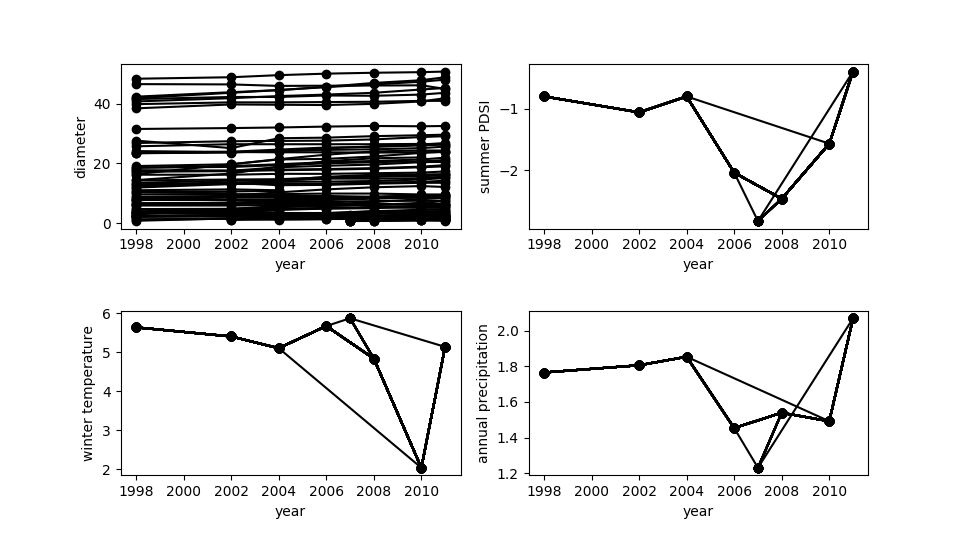
\includegraphics[width=1\textwidth]{diameter-weather.png}
    \caption{diameter measurement and weather factors for each individual}
    \label{fig:diameter-weather}
\end{figure}

We then construct the the weather records for all the years presented in the dataset, and figure ~\ref{fig:weather} presents the weather factors across the years. We notice that the summer PDSI and the annual precipitation present the same trend. To observe the correlation among the weather factors, we normalize their values and plot them in figure \ref{fig:normalized-weather}. We can see that the PDSI and precipitation are indeed highly correlated with correlation coefficient as hight as 0.93, while the correlation coefficient between PDSI and winter temperature is -0.04. So we will only take in two weather factors in our model development, i.e., the winter temperature with either summer PDSI or annual precipitation.

\begin{figure}[h!]
    \centering
    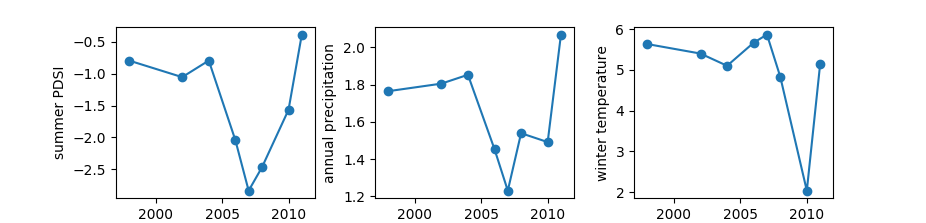
\includegraphics[width=1\textwidth]{weather.png}
    \caption{weather factors}
    \label{fig:weather}
\end{figure}

\begin{figure}[h!]
    \centering
    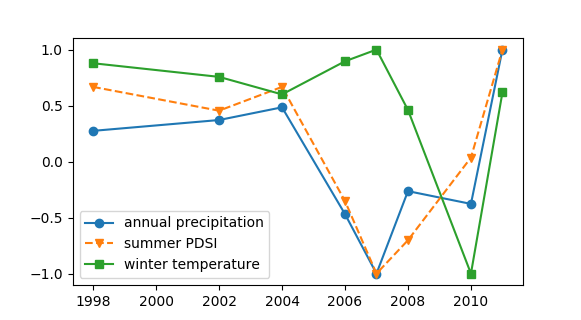
\includegraphics[width=0.5\textwidth]{normalized-weather.png}
    \caption{normalized weather factors}
    \label{fig:normalized-weather}
\end{figure}

Although all the observed trees have the same weather records that measured in the Duke Forest, in reality, however, trees may be distributed across the forest and thus have different environment. For example, they may receive different amount of sunshine in the day time and the soil condition may not be the same as well. So we cluster the trees manually by their growth trend. To better compare the growth trend of all trees, we deduct the diameter by the first measured diameter value for each tree, so we can see the growth in the observed time period clearly. There are 88 trees in the dataset, Figure \ref{fig:cm-initial-diff} shows the diameter changes since the first measurement. Notice that there are clear gaps in the figure and we can at least make three clusters. Besides, the diameter changes are dramatic for a few trees compared to others and look like outliers, so we remove them from the dataset (3 removed). We show the clustered and cleaned data in Figure ~\ref{fig:cm-initial-diff-clean-group}.

\begin{figure}[H]
    \centering
    \begin{subfigure}{.5\textwidth}
        \centering
        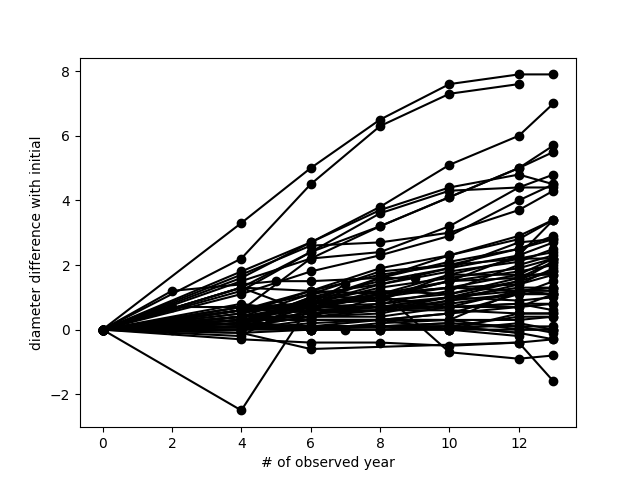
\includegraphics[width=1\textwidth]{cm-initial-diff.png}
        \caption{diameter change compared to first measurement}
        \label{fig:cm-initial-diff}
    \end{subfigure}%
    \begin{subfigure}{.5\textwidth}
        \centering
        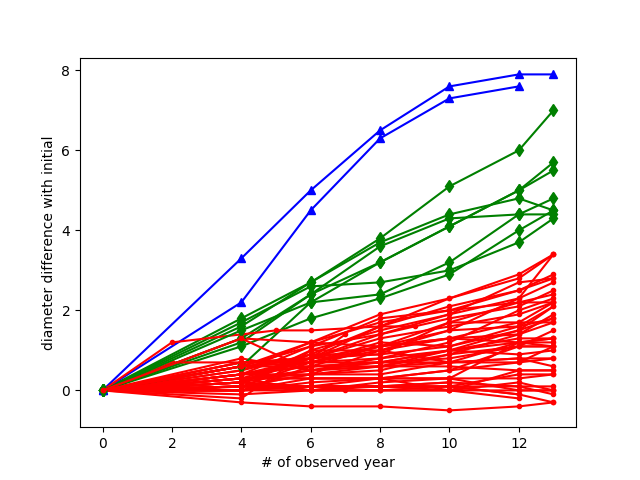
\includegraphics[width=1\textwidth]{cm-initial-diff-clean-group.png}
        \caption{clutter by growth trend}
        \label{fig:cm-initial-diff-clean-group}
    \end{subfigure}
\end{figure}

As we are studying the tree growth in terms of the diameter growth, we take the change in diameter since previous measurement and use it as the response variable in our model. Figure ~\ref{fig:cm-diff-scatter} shows the scatter plots of the diameter versus diameter change since laster measurement in each year. It is obvious that larger trees, i.e., trees that are larger in diameter, tend to have bigger growth. We also notice that the overall population growth slowed down slightly from year 2006 to year 2010, which is in correspondence with the drop down in summer PDSI and annual precipitation in those years as shown in Figure ~\ref{fig:weather}.

\begin{figure}[h!]
    \centering
    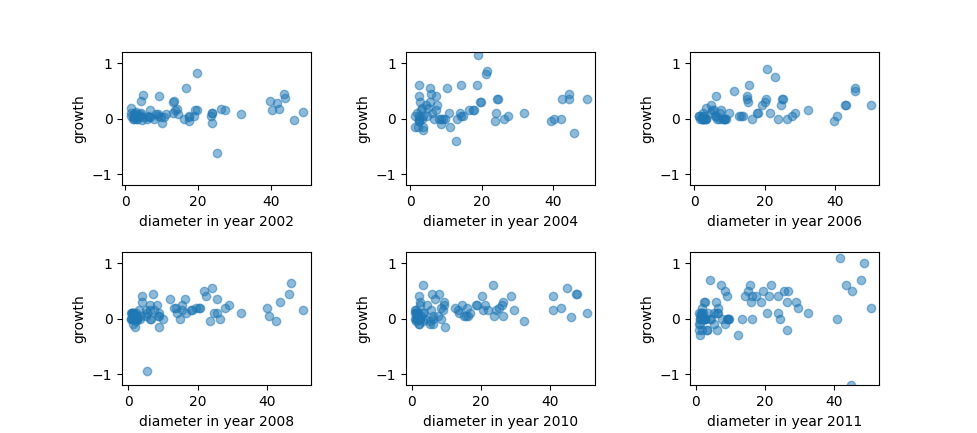
\includegraphics[width=1\textwidth]{cm-diff-scatter.png}
    \caption{growth scatter plot in different years}
    \label{fig:cm-diff-scatter}
\end{figure}

\section*{Model Development}

From now on, we will use the Wilkinson Notation \cite{wilkinson} to present the model formula. In our first model, annual diameter growth (denoted by $g$) is the response variable, and we use the diameter (denoted by $d$), the summer PDSI (denoted by $pdsi$) and the average winter temperature (denoted by $tmpr$) as the predictor variable, and the growth trend cluster (denoted by $cg$) as the grouping variable. Below is the formula $F1$:

\begin{align*}
    \textbf{F1}: g\sim1+d+pdsi+tmpr+(d|cg)+(pdsi|cg)+(tmpr|cg)
\end{align*}

We use the MATLAB function fitlme \cite{workflow} to fit the linear mixed-effects model which computes coefficients by maximum likelihood. With $F1$, The estimated standard deviations of $pdsi$ term and $tmpr$ term are nearly 0---3.36e-11 and 5.56e-12 respectively---and their confidence interval cannot be computed. This is an indication that the model is over parameterized and the $(pdsi|cg)$  term and $tmpr|cg)$ are not significant. We remove these two term and thus get the second model with the following formula:

\begin{align*}
    \textbf{F2}: g\sim1+d+pdsi+tmpr+(d|cg)
\end{align*}

The fitting with $F2$ is better than $F1$, as the BIC decreases by 6 and the p value for the estimation of coefficient of $d$ also decreases from 0.33 to 1.24e-06. But the p value for the estimation of coefficients of the $pdsi$ term and the $tmpr$ term are not convincing, with the first p value being 0.62 and the second being 0.24. We then try to remove these two term as well, arriving at formula $F3$:

\begin{align*}
    \textbf{F3}: g\sim1+d+(d|cg)
\end{align*}

The result is promising, as the BIC value further drops by 10 and the p value for the estimation of the two fixed effect coefficients (the intercept and the $d$ term) are 0.037 and 1.123e-06 respectively. The effects of weather factors on tree growth are ignored in the last model which may be disturbing, but if we look deep at figure ~\ref{fig:cm-initial-diff-clean-group}, only a few trees presented significant drop in growth in the observed year 3 to year 6 when the population were experiencing moderate summer drought, and it's probably that the effects of weather is not significant enough in the observed time span. Actually, when we investigate how many trees had slowed down growth rate compared to the former measurement in the year of 2006 when they were undergoing the most severe summer drought recorded in the dataset, results show that only 44\% of the population were under impact. We present the final model in the following tables.

\begin{table}[h!]
    \centering
    \begin{tabular}{ |c | c | c | c | } 
        \hline
        AIC& BIC & LogLikelihood & Deviance\\ 
        \hline
        -114.47 & -87.482 & 64.234 & -128.47 \\ 
        \hline
        \end{tabular}
    \caption{Model Fit Statistics}
\end{table}

\begin{table}[h!]
    \centering
    \begin{tabular}{ |l | c | c | c | c | } 
        \hline
        Name& Estimate & pValue & Lower & Upper\\ 
        \hline
        Intercept & 0.069 & 0.037 & 0.004 & 0.134\\
        \hline
        $d$ & 0.006 & 1.125e-06 & 0.004 & 0.009\\
        \hline
        \end{tabular}
    \caption{Fixed Effects Coefficients (95\% CIs)}
\end{table}

\begin{table}[h!]
    \centering
    \begin{tabular}{ |l | l | c | c | c | c |} 
        \hline
        \multicolumn{6}{|c|}{Group: $gc$ (3 Levels)} \\
        \hline
        Name1 & Name2 & Type & Estimate & Lower & Upper\\ 
        \hline
        Intercept & Intercept & std & 0.049 & 0.017 & 0.138\\
        \hline
        $d$ & Intercept & corr &  -1 & NaN & NaN \\
        \hline
        $d$ & $d$ & std & 0.002 & 0.000 & 0.010 \\
        \hline

        \multicolumn{6}{|c|}{Group: Error} \\
        \hline
        \multicolumn{3}{|l|}{Name} & Estimate & Lower & Upper \\
        \hline
        \multicolumn{3}{|l|}{Res Std} & 0.200 & 0.186 & 0.216 \\
        \hline
        \end{tabular}
    \caption{Random Effects Covariance Parameters (95\% CIs)}
\end{table}

\section*{Conclusion}

In this study, we investigate how weather factors such as PDSI, annual precipitation and winter temperature may affect the tree growth rate. We find that, as far as the recorded data are considered, the winter temperature has very limited effect on tree growth rate. And while the summer PDSI does have some negative effects on some trees, more than half of the observed population are no affected. Overall, under the weather condition recorded in the dataset, a tree's growth rate is dominated by its current size. 


\bibliography{project3} 
\bibliographystyle{ieeetr}
\end{document}

